%%%%%%%%%%%%%%%%%%%%%%%%%%%%%%%%%%%%%%%%%%%%%%%%%%%%%%%%%%%%%%%%%%%%%%%%%%%%%%%%
%2345678901234567890123456789012345678901234567890123456789012345678901234567890
%        1         2         3         4         5         6         7         8
\documentclass[a4paper, 10pt, conference]{ieeeconf}      % Use this line for a4 paper

\IEEEoverridecommandlockouts                              % This command is only needed if 
                                                          % you want to use the \thanks command

\overrideIEEEmargins                                      % Needed to meet printer requirements.

% See the \addtolength command later in the file to balance the column lengths
% on the last page of the document

\usepackage[utf8x]{inputenc}

\usepackage[protrusion=true,expansion=true]{microtype}
\usepackage{cite}
\usepackage{graphicx}
\usepackage{hyperref}
\usepackage{url}
\usepackage{amsmath}

\usepackage[cache]{minted}
\renewcommand{\theFancyVerbLine}{
  \sffamily\textcolor[rgb]{0.5,0.5,0.5}{\scriptsize\arabic{FancyVerbLine}}}

\newminted{python}{frame=lines,
                    linenos=true,
                    gobble=4,
                    fontsize=\scriptsize,
                    xleftmargin=1.8em}

\newmintinline[python]{python}{fontsize=\footnotesize}

\graphicspath{{figs/}}
\DeclareGraphicsExtensions{.pdf,.jpg,.png}

\usepackage[draft]{fixme}

\newcommand{\ie}{{\textit{i.e.\ }}}
\newcommand{\cf}{{\textit{cf\ }}}
\newcommand{\eg}{{\textit{e.g.\ }}}
\newcommand{\pyRobots}{\textsc{pyRobots}\ }


\title{\LARGE \bf
    \pyRobots, a toolkit for robot executive control
}

\author{Séverin Lemaignan, Anahita Hosseini and Pierre Dillenbourg\\
Computer-Human Interaction in Learning and Instruction \\
École Polytechnique Fédérale de Lausanne (EPFL) \\
CH-1015 Lausanne, Switzerland \\
{\tt\small firstname.last@epfl.ch}
}

\begin{document}


\maketitle
\thispagestyle{empty}
\pagestyle{empty}


%%%%%%%%%%%%%%%%%%%%%%%%%%%%%%%%%%%%%%%%%%%%%%%%%%%%%%%%%%%%%%%%%%%%%%%%%%%%%%%%
\begin{abstract}

    Blabla

\end{abstract}


%%%%%%%%%%%%%%%%%%%%%%%%%%%%%%%%%%%%%%%%%%%%%%%%%%%%%%%%%%%%%%%%%%%%%%%%%%%%%%%%
\section{Introduction}

Orchestrating the activity of a robot is a central issue of robotics: \emph{what
to do when?} Traditionally, in the famous 3-layer architectures~\fixme{ref?},
this function is implemented in the so-called \emph{deliberative layer} where
decisions are made based on perceptions and on the current internal state, and
executed by sending orders to a \emph{functional layer}.

While individual decision-making components (like task planners) are studied in
(relative) isolation since years, the \emph{orchestration} issue, with questions
like \textit{When to start them? Which one should be selected? How to react to a
new situation in a timely manner?} remains difficult to address in a generic
way.

Many approaches have been devised (we review them in the next section) that
include \emph{Finite State Machines} (FSM), domain-specific languages (in
particular, logic languages) or agent-based frameworks.

These tools adopt principled approaches, often with solid theoretical
contributions. However, it seems that none of them gained broad acceptance in
the robotic community, and many of us resort to write ad-hoc scripts, suitable
for a single application/demonstration/experiment and neither reliable nor
extensible.

We hypothesize that the software architecture design that these tools enforce,
combined with their general lack of practicality (unfamiliar language; lack of
bindings for a given robot or middleware; difficulty to install or setup;
non-trivial deployment) explain this low level of acceptance more than any
particular intrinsic weaknesses.

This article introduces our attempt at designing an unobtrusive execution control
toolkit, that aims at addressing the \emph{practicality} issue: it has been
designed and implemented from the bottom-up, starting from actual needs when
running complex robots in largely unpredictable scenarios (typically,
loosely constrained human-robot interactions), and in the real world.

Instead of an \emph{environment} or a \emph{framework}, which would suggest
strong design and development constraints, \pyRobots can be conceived as a set of
powerful software helpers to write parallel, event-based, high-level robot
controllers.

It is written for and in Python, which ensure familiarity, fast development
cycles and broad support for interfacing with existing robots and middlewares.
This must be emphasized: \pyRobots is \emph{not} a middleware. It purposefully
provides no mechanisms to connect to other modules or components. It instead
\emph{uses} one (or several) middleware to actually communicate with the robot
and perform actions.

One the other hand, \pyRobots does not provide formal models or verifiability:
in its current state, it does not attempt to contribute in this field. It
focuses instead on providing unobtrusive tools to control robots in environments
that require carrying out many tasks in parallel, in an unpredictable,
event-based manner.

\subsection{Related Work: Robot Execution Control}

Any robotic experiment requires a certain amount of high-level control to
supervise the robot behaviour, and, expectedly, many projects have attempted to
design and provide tools for this task.  We focus this review on \emph{tools
dedicated to the explicit implementation of high-level behaviours}, excluding
complete control stacks (that would typically include a middleware and hardware
abstractions), meta-tools (like component generators or model checkers) and
(semi-)automatic techniques (like learning by demonstration).  In contrast with
middlewares for which the robotic community relies on a few \emph{de-facto}
standards (ROS, YARP, OpenRTM), we want to underline that no such widely-used
softwares exist for execution control, and we believe that most of today's robot
behaviours are implemented as \emph{ad-hoc} scripts.

We identify three categories of execution control tools: \emph{finite state
machines}, \emph{agent-based} controllers and
\emph{domain-specific languages} (DSL), including \emph{embedded domain-specific
languages} (eDSL,~\cite{joyeux2011robot}). These categories overlap to a certain
extend, but they should reasonably reflect the motivational concepts/ideas that
gave birth to the specific tools.

\paragraph{Finite State Machines} (or FSM) are the most well-known paradigm to
describe how a robot goes from one \emph{state} (typically, performing an
action) to another state when some condition becomes true or some event is
triggered. Common FSM implementations in robotics include {\sc
rfSM}~\cite{klotzbucher2010orocos} (part of the OROCOS framework) and
{\sc smach}~\cite{bohren2010smach}. State machine semantics are well
understood~\cite{harel1996statemate} and provide a well structured model,
suitable for meta-reasoning (like verification). However, FSM are also
acknowledged to be ill-suited for complex systems (where the number of state
easily ``explodes'') or relatively dynamic and unpredictable environments where
it can prove difficult to \textit{a priori} exhaustively list transitions.


\paragraph{Agent-based controllers}

temporal planning/temporal constraints: T-REX~\cite{mcgann2007trex} -> sensing-planning-acting

ROAR: ~\cite{degroote2011roar}

\paragraph{Domain-specific languages}

Domain-specific languages (DSL), in the widest sense, represent the largest body
of literature on high-level behaviour programming. They can either be ``actual''
domain-specific languages like PRS~\cite{ingrand1996prs},
RPL~\cite{mcdermott1993reactive}, Golog~\cite{levesque1997golog} (and its
derivative like {\sc ReadyLOG}~\cite{ferrein2007robot} or, more recently,
URBI~\cite{baillie2005urbi}; or what Joyeux calls \emph{embedded}
DSL~\cite{joyeux2011robot}: extensions of existing languages (typically, dynamic
languages like Python or Ruby, or logic languages like Prolog) to provide
high-level paradigms and control structures well suited to the programming of
robots. {\sc cram}~\cite{beetz2010cram} (based on Lisp and Prolog), {\sc
roby}~\cite{joyeux2009plan} (based on Ruby), {\sc
teer}~\footnote{\url{http://wiki.ros.org/executive_teer}} (based on Python), are
examples of such eDSL.

Projects like PRS, Golog or {\sc cram} have large scopes:


\pyRobots positions itself in this landscape as a lightweight eDSL (in a similar
fashion to {\sc roby} or {\sc teer}), that focuses on high-level behaviours
implementation. It seeks unobstrusive interaction with the other components of
the robot software stack, using Python as ubiquitous binding language. Similar
to URBI, it focuses on transparent preemptive concurrency and event-based programming.
Also, \pyRobots' model favours hierarchical task composition over plans, and does not
provide by itself any task planning service, delegating this to external tools.

\subsection{Guiding principles}

\begin{itemize}
    \item Use a de-facto standard language (Python) to ease adoption (familiar to
        many researchers, large software ecosystem, excellent integration with
        most robotic softwares, in particular common middlewares like ROS or
        YARP)
    \item should be as lightweight/transparent as possible (in particular from a
        syntax perspective) so that the
        programmer can focus on the programming of the behaviours (I'm
        watching you, SMACH)
    \item should enforce as few design choices as possible. 'convention over
        configuration' as often as possible
\end{itemize}

\subsection{Main features}

Parallelism (all \emph{actions} are asynchronous) and event-based programming
are at the core.

It also offers support for robot resources management (locking of ``parts'' of
the robot) and uniform manipulation of 6D poses (that integrates transparently
with other tools like ROS's TF when available).

\section{Concepts and Overview}

Before introducing and explaining step-by-step a complete working example in the
next section, it is useful to first introduce the main concepts of \pyRobots,
and provide an overview of the features and mechanisms. Since \pyRobots is an
open-source software, the interested reader can also refer to the source code,
available here:~\url{https://github.com/chili-epfl/pyrobots}.

\begin{itemize}
    \item Lock specific resources with a simple \python|@lock(...)| in front of the
        actions. When starting, actions will wait for resources to be
        available if needed.
    \item Supports compound resources (like \python|WHEELS == LEFTWHEEL + RIGHTWHEEL|)
    \item Poses are managed explicitly and can easily be
        transformed from one reference frame to another one
        (integrates with ROS TF when available).
    \item Extensive logging support to debug and replay
        experiments.
\end{itemize}

\subsection{Core concepts}

\pyRobots core concepts are simple: on one hand, the user creates a
\textbf{robot} as an instance of a \python|GenericRobot|, that encapsulates the
different low-level \textbf{controllers} (proxies to actuators, typically
provided by a middleware like ROS) and the \textbf{state} of the robot
(typically a set proxies to the sensors, or a connector to a database, etc.,
accessed through a dictionary-like object).

On the other hand, the user creates as many high-level \textbf{actions} as
desired, as regular Python functions. Actions are automatically added to the
\textbf{robot}, and can access its state and controllers to perform actual
physical actions.

The user can list \textbf{events} that the \textbf{robot} must monitor, and
attach callback to them.

Finally, the user can declare arbitrary \textbf{resources}, usually
corresponding to the robot components (for instance, the wheels, the camera,...)
and guarantee exclusive access to the required resource to specific actions.

\subsection{Asynchronous actions}

\emph{Actions} in \pyRobots are always asynchronous. They are implemented as
\emph{futures} (also known as \emph{promises}) and therefore executed in
independent threads. To the developer, however, they appear as regular Python
function, simply annotated with the \python|@action| decorator, and are invoked
like any other function.  Since they are asynchronous, these functions may
perfectly block or even never return (typically useful to implement lasting
background behaviours).

Actions can also call each other, allowing natural decomposition of complex
tasks into sub-actions and atomic actions.

\paragraph{Signaling} Behaviours often need to be paused of cancelled.  This
raises an issue that needs to be addressed in robotics: before suspending an
action, one often wants to first bring back the robot into some form of rest
state (\eg one would not want to suddenly cancel a \python|walk| action in the
middle of a step without first bringing back the foot to the ground).

\pyRobots addresses this issue through signals, and extends standard
Python thread into \emph{signaling threads}, relying on Python's usual syntax
for exception handling. Listing~\ref{lst:signals}
illustrates this mechanism. The action is instantiated and started at line 8,
and cancelled at line 10. This send a \python|ActionCancelled| signal to the
action that the user can handle using an \python|except| statement.

\begin{listing}[H]
\begin{pythoncode}
    @action
    def my_action(robot):
      try:
        robot.do_something_long()
      except ActionCancelled:
        robot.go_back_to_rest_pose()

    action = robot.my_action()
    time.sleep(1)
    action.cancel()
\end{pythoncode}
\caption{Handling a cancellation signal}
\label{lst:signals}
\end{listing}

Pausing actions is more complex (the action internal state must be saved, a mean
to resume the action where it was interrupted must be provided, the user must be
given ways to code transition behaviours when pausing and resuming) and is not
currently supported by \pyRobots.

\subsection{Events}

Sharing the same syntax with URBI, events in \pyRobots can by monitored through
the methods \python|on| (one shot event) and \python|whenever| (continuous event
monitoring). Event conditions can be either a predicate (that must take as
single argument the robot instance) or a pair of $\{\text{state member},
\text{condition}\}$ with condition in $\{\text{value}=x, \text{become}=x,
\text{below}=x, \text{above}=x, \text{decrease}=x, \text{increase}=x\}$. An
example of event usage can be seen at line 67 of listing~\ref{mwe}.

When the event condition is verified, the callback (usually, an action) is
invoked from the event monitor thread.

\subsection{Resources management}

Usually, physical robot resources (mainly actuators, but possibly sensors as
well) require exclusive use (it is seldom desirable that two different actions
control the wheels of a robot at the same time). 

To leave full control regarding the required resource modeling granularity, the
programmer define them himself, either as stand-alone resources or as compound
resources (listing~\ref{lst:resources}).

\begin{listing}[H]
\begin{pythoncode}
    L_ARM = Resource()
    R_ARM = Resource()
    ARMS = CompoundResource(L_ARM, R_ARM)

    @action
    @lock(ARMS)
    def lift_box(robot):
        #...

    @action
    @lock(L_ARM)
    def wave_hand(robot):
        #...

    @action
    @lock(L_ARM, wait=False)
    def scratch_head(robot):
        #...

    robot.lift_box()
    robot.wave_hand() # waits until lift_box is over
    robot.scratch_head() # skipped if lift_box 
                         # is still running

\end{pythoncode}
\caption{Resource usage is defined at the action-level, through annotations.}
\label{lst:resources}
\end{listing}

The user then annotates the actions with the (possibly multiple) resources they
require (lines 6, 11 and 16 of listing~\ref{lst:resources}). When executed, the
action acquires a lock on the resource (and all dependent resources in the case
of a compound resource) which is released upon action completion. In the
meantime, other actions requiring the same resource will either wait until the
resource is release (line 21) or be skipped (line 22) if the \python|@lock|
annotation specifies not to wait (line 16).


\subsection{Uniform management of poses and rigid transformations}

Managing poses, transformations, frames in real-world scenarios is not an easy
task, mainly because it seems that every single library, middleware or robotic
platform rely on its own conventions (rotation representations, in particular,
are a constant source of frustration, having to jump all the time between
quaternions, one of the 23 Euler conventions, rotation matrices, Rodrigues,
yaw-pitch-roll notation...). Within the ROS ecosystem, the Transform Library
(tf,~\cite{foote2013tf}) has played a major role to make it convenient to work
with frames, and poses can always be expressed and shared in the most convenient
local frame, tf taking care of required intermediate transformation.

\pyRobots offers a similar approach \emph{within} the control script, adding a
pinch of syntactic sugar to make poses and frame management transparent for the
high-level action controller.

As illustrated in listing~\ref{lst:poses}, poses can be flexibly defined by a
simple frame name, by a triple $\{x, y, z\}$ (default frame {\tt map} is then
assumed), by a 4-tuple $\{x, y, z, frame\}$, by a 6-tuple $\{x, y, z, rx, ry,
rz\}$ (using $sxyz$ Euler convention), by a 7-tuple $\{x, y, z, rx, ry, rz,
frame\}$, by a 7-tuple $\{x, y, z, qx, qy, qz, qw\}$, by a 8-tuple $\{x, y, z,
qx, qy, qz, qw, frame\}$ or by a dictionary that defines any of these 8 values.
Internally, \pyRobots normalizes and stores the poses in their full 8-tuple
expansion.

\begin{listing}[H]
    \begin{pythoncode*}{linenos=false, xleftmargin=0em}

    robot.poses["handL"]
    # -> {'x':0., 'y':0., 'z':0., 
    #    'qx':0., 'qy':0., 'qz':0., 'qw':1., 
    #    'frame': 'handL'}

    robot.poses[(1.0, 0.0, 0.0)]
    # -> {'x':1., 'y':0., 'z':0., 
    #    'qx':0., 'qy':0., 'qz':0., 'qw':1., 
    #    'frame': 'map'}

    robot.poses[{'z':1.0, 'rz':0.2, 'frame':'handL'}]
    # -> {'x':0., 'y':0., 'z':1., 
    #    'qx':0., 'qy':0., 'qz':0.0998, 'qw':0.0995, 
    #    'frame': 'handL'}

\end{pythoncode*}
\caption{Examples of pose normalization.}
\label{lst:poses}
\end{listing}

Using helper methods like \python|robot.poses.inframe(<pose>, <other frame>)| or
\python|robot.poses.pantilt(<pose>, <ref frame>)|, the programmer can then
transform a given pose into a different frame or different representation.

These transformations are directly computed, but \pyRobots also takes advantage
of middleware-specific infrastructure (when available) to provide known frames.
ROS TF, Aldebaran's {\tt NAOqi} frame conventions, etc. are used when available
through specializations of the \pyRobots \python|PoseManager| class.

\subsection{Developer support: logging, debugging, introspection}
\label{}

Running robots in real-world, \ie dynamic and unpredictable, environments
entails repetitive coding-testing-debugging development cycles. \pyRobots
provides several tools to support this development phase. A special attention
was paid to the logging infrastructure. It relies on the versatile Python
built-in logging tools, which support configurable parallel logging streams
(typically, a full debug stream is logged to a file while a less verbose stream
is output on the console at run-time).

\pyRobots logs are designed to allow full \emph{post-mortem} replay, and we
provide a graphical interface to display the actions and resource usage over
time (Figure~\ref{log_view}).

\begin{figure}
        \centering
        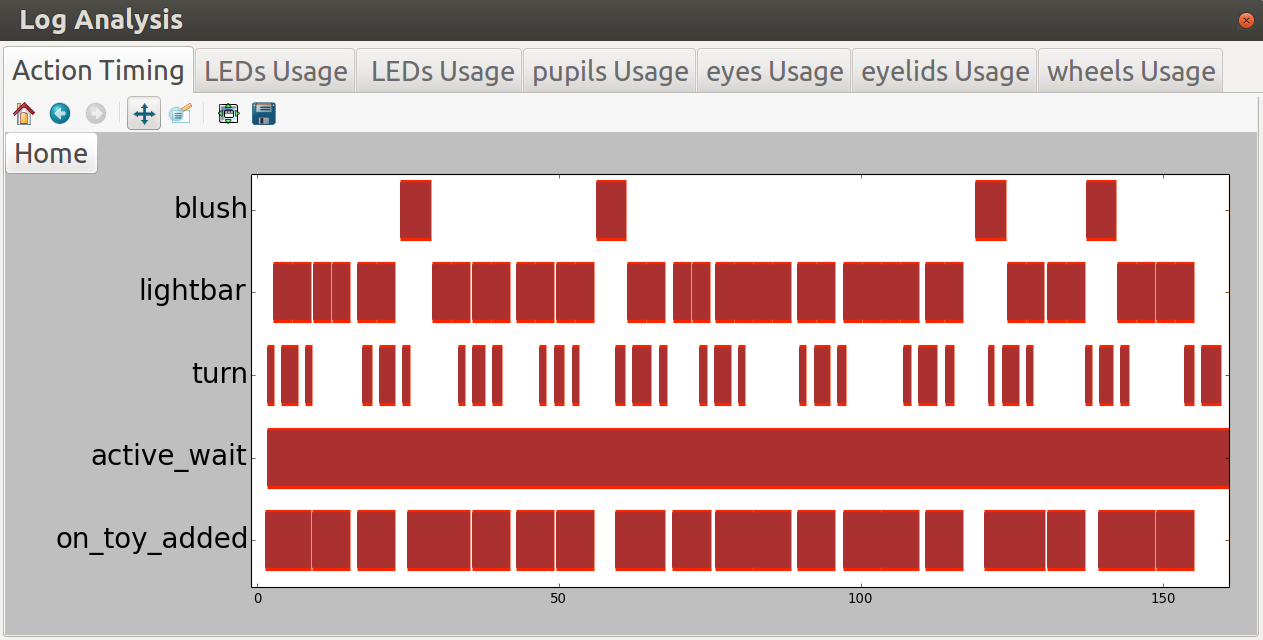
\includegraphics[width=0.9\columnwidth]{log}
        \caption{Screenshot of \pyRobots log analyser, processing the log of the
        experiment presented at section~\ref{croq}}
        \label{log_view}
\end{figure}

Debugging and introspection support is provided at run-time through a range of
off-the-shell Python debuggers. Remote debugging is also supported with standard
tools like {\sc rpdb2}~\footnote{\url{http://winpdb.org}}. Thanks to the dynamic
nature of Python, these debuggers not only provide insights on failures, but
also provide full introspection and run-time manipulation of the application
state.

%%%%%%%%%%%%%%%%%%%%%%%%%%%%%%%%%%%%%%%%%%%%%%%%%%%%%%%%%%%%%%%%%%%%%%%%%%%%%%
\section{Detailed Example}

\begin{listing}[h!]

\begin{pythoncode}
    import time
    from robots import GenericRobot
    from robots.decorators import action, lock
    from robots.resources import Resource
    from robots.signals import ActionCancelled

    # create a 'lockable' resource for our robot
    WHEELS = Resource("wheels")

    class MyRobot(GenericRobot):

      def __init__(self):
        super(MyRobot, self).__init__()

        # create (and set) one element in the robot's state.
        # Here a sonar.
        self.state["sonar"] = 10.

        # do whatever other initialization you need :-)

      def send_goal(self, pose):
        # move your robot using your favorite middleware
        print("Starting to move towards %s" % pose)

      def stop(self):
        # stop your robot using your favorite middleware
        print("Motion stopped")

      def whatever_lowlevel_method_you_need(self):
        pass

    @lock(WHEELS)
    @action
    def move_forward(robot):
      """ Actions are written in a simple imperative, 
          blocking style.
      """

      # the target pose: simply x += 1.0m in the robot's 
      # frame. pyRobots will handle the frames 
      # transformations as needed.
      target = [1.0, 0., 0., "base_link"]

      try:
        robot.send_goal(target)

        while(robot.pose.distance(robot.pose.myself(), 
                                  target) > 0.1):
            # robot.sleep is exactly like time.sleep, 
            # except it lets the pyrobots signals pass 
            # through.
            robot.sleep(0.5)

        print("Motion succeeded")

      except ActionCancelled:
        # if the action is cancelled, clean up your state
        robot.stop()


    with MyRobot() as robot:

      # Turn on DEBUG logging.
      # Shortcut to configure the std Python logging system
      robot.debug()

      robot.whenever("sonar", below = 0.3).do(move_forward)

      try:
        while True:
          time.sleep(0.5)
      except KeyboardInterrupt:
        pass
\end{pythoncode}
\caption{Full example of a \pyRobots application.}
\label{mwe}
\end{listing}


\section{Experimental Deployments}

The development of \pyRobots started in 2011, driven by the requirements of a
18-min long theatre performance between a human actor and a robot. Since that time, the toolkit has
iteratively matured, and has been deployed and used on several projects and
platforms. We first briefly recap these deployments with references to the
corresponding publications, and then present our latest study, in a nursery,
that recently acted as a stress-test for the library.

%%%%%%%%%%%%%%%%%%%%%%%%%%%%%%%%%%%%%%%%%%%%%%%%%%%%
\begin{table}[ht!]
\begin{center}
\begin{tabular}{p{0.9\columnwidth}}
\hline
    {\bf Manipulation} \\
     {\tt attachobject}, {\tt basicgive}, {\tt basictake}, {\tt close\_gripper}, {\tt configure\_grippers}, {\tt grab\_gripper}, {\tt handover}, {\tt hide}, {\tt open\_gripper}, {\tt pick}, {\tt put}, {\tt put\_accessible}, {\tt release\_gripper}, {\tt show}, {\tt take} \\
\hline
    {\bf Gaze control} \\
     {\tt glance\_to}, {\tt look\_at}, {\tt sweep}, {\tt switch\_active\_stereo\_pair}, {\tt track}, {\tt cancel\_track} \\
\hline
    {\bf Navigation} \\
     {\tt carry}, {\tt follow}, {\tt cancel\_follow}, {\tt goto}, {\tt moveclose}, {\tt waypoints} \\
\hline
    {\bf Local navigation} \\
     {\tt dock}, {\tt rotate}, {\tt translate} \\
\hline
    {\bf Posture configuration} \\
     {\tt extractpose}, {\tt idle}, {\tt manipose}, {\tt movearm}, {\tt rest}, {\tt setpose}, {\tt settorso}, {\tt tuckedpose} \\
\hline
\end{tabular}
\end{center}
\caption{Examples of \pyRobots actions, mostly extracted from experiments involving
    the PR2 robot.}

\label{pyrobots_actions}
\end{table}
%%%%%%%%%%%%%%%%%%%%%%%%%%%%%%%%%%%%%%%%%%%%%%%%%%%%


\paragraph{Roboscopie} The first complex deployment scenario for \pyRobots was
indeed a theatre performance entitled
\emph{Roboscopie}~\cite{lemaignan2012roboscopie}. The toolkit was created out of
the need to control a complex robot (a Willow Garage PR2) in a structured way,
as required for a live performance with a human\footnote{The original \pyRobots
script used for the performance can be accessed
from~\url{http://www.laas.fr/roboscopie}. Note that this script does not
reflect anymore the toolkit usage.}

A total of 47 \pyRobots actions were written for this event
(Table~\ref{pyrobots_actions} gives a few examples), and the toolkit proved to
be especially convenient to interleave calls to both ROS-based and {\sc
GenoM}-based\footnote{{\sc GenoM} is software component as well as a middleware
developed at LAAS-CNRS} components through their respective Python bindings.

\pyRobots also allowed us to retain the \emph{rapid prototyping} convenience of a
script language, essential for the robot to ``practise'' and adapt to the
vision of the director.

\begin{itemize}
    \item PR2, with ROS and pocolibs
    \item Nao, with ROS and NAOqi
    \item Ranger with Aseba and ROS
\end{itemize}


\begin{itemize}
    \item roboscopie
    \item LAAS architecture
    \item CoWriter
    \item Ranger
\end{itemize}

\begin{figure}
        \centering
        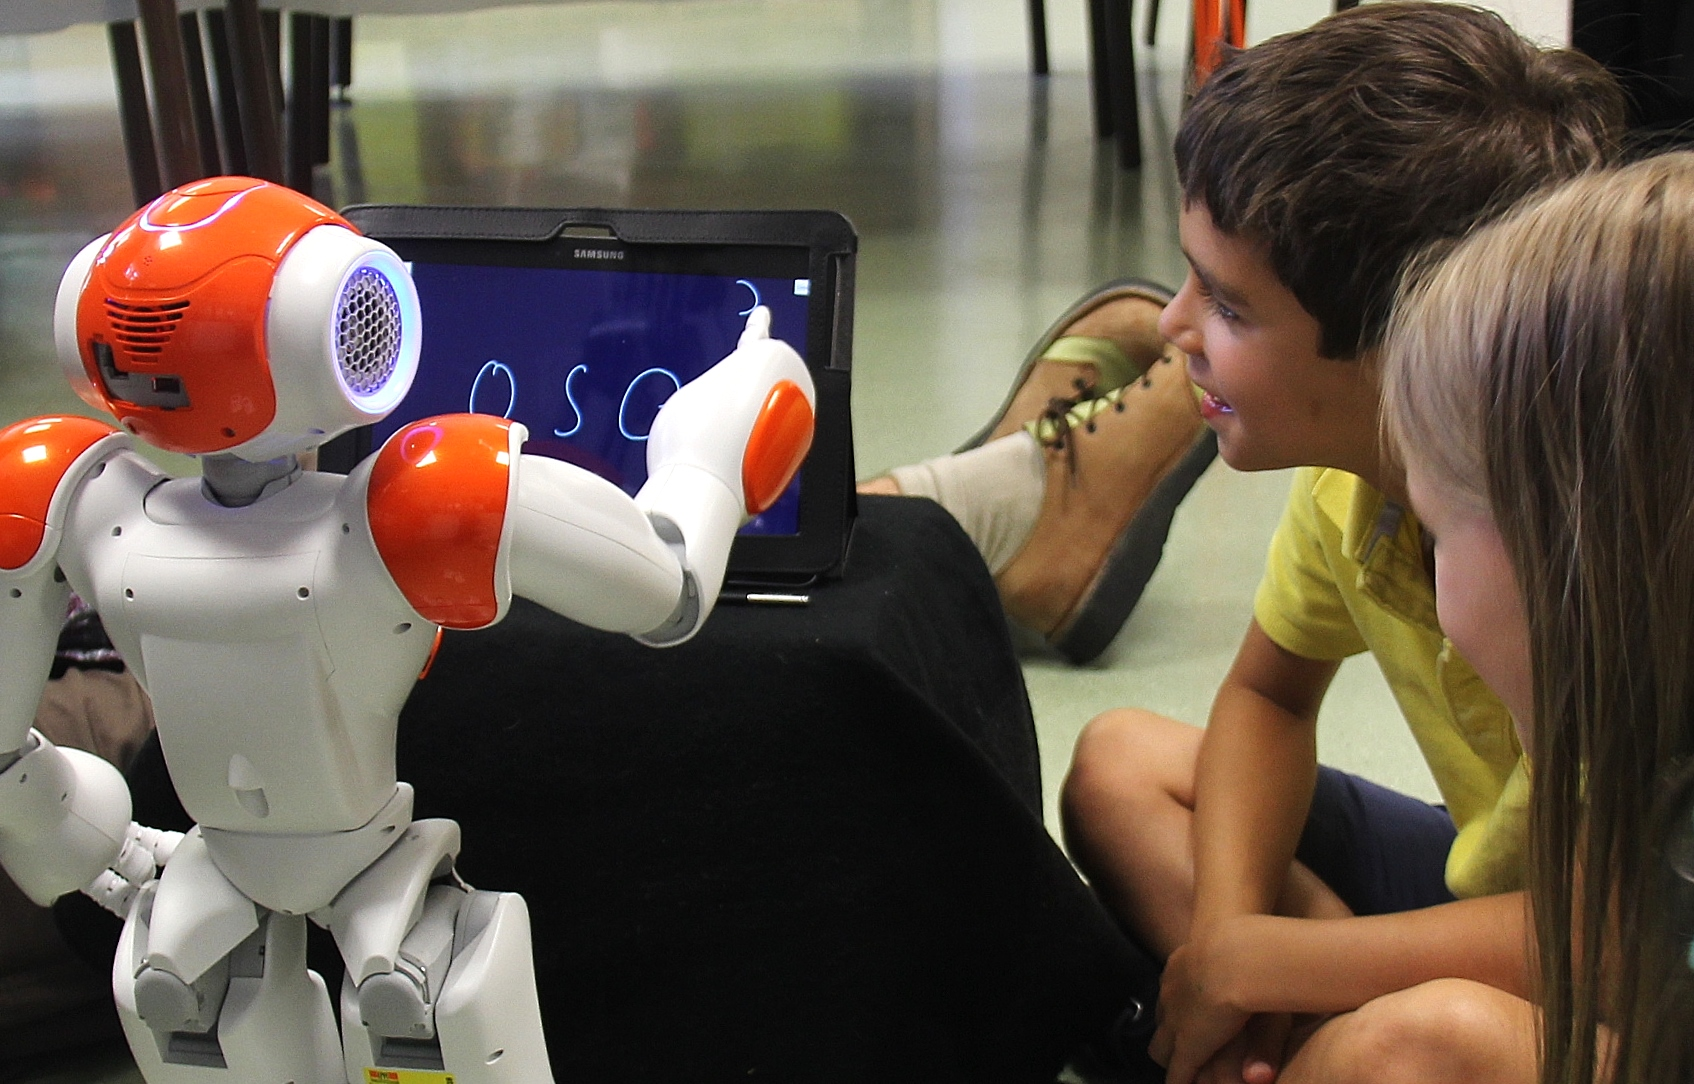
\includegraphics[width=0.9\columnwidth]{cowriter}
        \caption{Children teaching an Aldebaran Nao interacting how to
        handwrite.}
        \label{expe-cowriter}
\end{figure}

\paragraph{Stress-test in a nursery}
\label{croq}

We organized in June 2014 a pilot study in a kindergarten (on campus) to
stress-test the hardware and software of the Ranger
robot~\cite{mondada2014ranger}. The Ranger robot is an autonomous robot designed
for interaction with children. As it was primarily designed to support children
with tidying up, it is shaped as a wooden ``box on wheels''
(Figure~\ref{expe-nursery}). Hardware-wise, it features an RGB-D camera, IR
sensors, a range and bearing sensor, a physical front bumper, a scale, a
removable pacifier (used as a soft on/off switch by the children) and it is
covered with capacitive tactile panels. The wooden panels cover 186 RGB LEDs,
enabling various light patterns, it can play sounds, the two eyes can be fully
controlled (2 DoFs pupils and actuated eye-lids). Wheel controllers are designed
such as they switch to freewheel as soon as the robot is pushed by the children.
The robot is powered by an embedded Gumstix Overo (ARM7l) board running a custom
Linux image, assisted by three custom microcontroller boards (for low-level
hardware interfacing).

Software-wise, all the user-facing behaviours are implemented with \pyRobots,
and the communication with the hardware is abstracted through a mix of ROS
and Aseba~\cite{magnenat2011aseba} nodes.

\begin{figure}
        \centering
        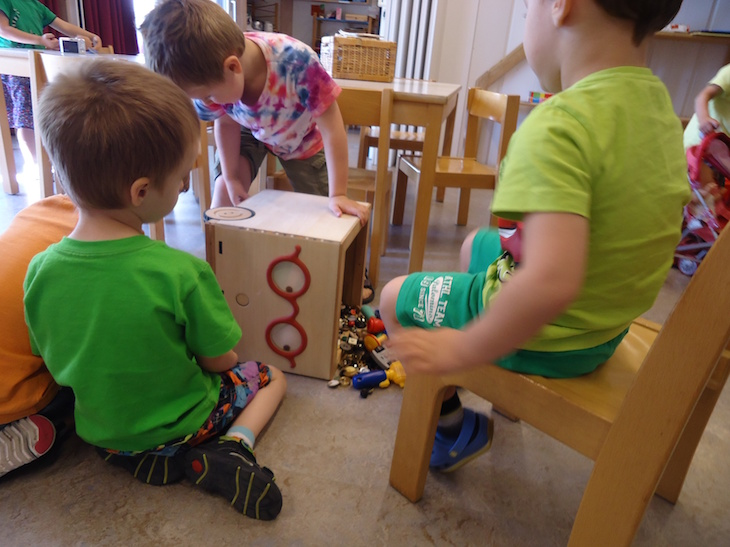
\includegraphics[width=0.9\columnwidth]{ranger-side}
        \caption{Infants playing freely (!) with an EPFL's \emph{Ranger} robot.
        The behaviour of the robot is controlled with \pyRobots.}
        \label{expe-nursery}
\end{figure}

We brought two Ranger robots to a kindergarten (17 children, mean age: 3.88
years old, SD=0.65), and after a brief introduction (showing them that removing
the pacifier would ``wake up'' the robot, and putting it back would make it
``fall asleep''), we invited the children to freely play with the robots and
integrate them into their usual games. The experiment lasted 68 minutes.

We purposefully designed a simple behavioural scheme
(Listing~\ref{croquignole_no_move}): two background actions
(\python|background_blink| and \python|look_at_touches|) run continuously, and 4
events are monitored (pacifier added/removed, toy added and bumper hit).

\begin{listing}[h!]

\begin{pythoncode}
    @action
    def on_pacifier(robot):
        robot.look_at_lolette()
        robot.blink()
        sleep = robot.fall_asleep()
        robot.lightbar(ramp=colors.RAINBOW).wait()
        sleep.wait()
    
    @action
    def on_pacifier_removed(robot):
        robot.light_bar(colors.from_hls(rand(0,1),0.8,1))
        robot.wakeup().wait()
        robot.move(0.4, v = 0.8).wait()
        robot.idle().wait()
    
    @action
    def on_bumper(robot):
        pulse = robot.pulse_row(0, (128, 0, 128))
        while abs(robot.state.v) > 0.01:
            robot.sleep(0.2)
        pulse.cancel()
    
    @action
    def on_toy(robot):
        robot.playsound(SOUNDS["toy_in"])
        robot.lightbar(ramp=colors.RAINBOW).wait()
    
    with Ranger() as robot:
    
        robot.background_blink()
        robot.look_at_touches()
    
        robot.every("pacifier", becomes = True).do(on_pacifier)
        robot.every("pacifier", becomes = False)
                                       .do(on_pacifier_removed)
        robot.every("scale", increase = 0.3).do(on_toy)
        robot.every("bumper", becomes = True).do(on_bumper)
    
        while True:
            time.sleep(0.1)
\end{pythoncode}
\caption{Source of the high-level behaviours running on the robots during the
nursery pilot (some behaviours like battery management have been omitted for
clarity).}
\label{croquignole_no_move}
\end{listing}



\begin{figure}
    \resizebox{\columnwidth}{!}{\input{croquignole-expe}}
    \caption{Events fired and actions started per minute, over the 68 min-long
    experiment. The robot sustains an average of 70 actions triggered by minute over
    more than an hour, with peaks at 200 actions/minute.}

\end{figure}

\section{Conclusion and Future Work}

\subsection{Summary and main contributions}

\begin{itemize}
    \item strives to simplicity (from a user perspective)
    \item Middleware independent, real-world deployments with with ROS, GenoM, NAOqi, aseba
\end{itemize}

\subsection{Future work}

\begin{itemize}
    \item control mixing policies?
    \item control over action priorities
    \item path to more complex control tool (T-REX, etc)
\end{itemize}

\section*{Acknowledgment}

This work has been supported by...

\bibliographystyle{IEEEtran}
\bibliography{pyrobots}


\end{document}
